\chapter{Generaci\'on de expresiones referenciales}
\label{sec:seleccion}

En este cap\'itulo presentamos definiciones b\'asicas y un resumen del estado del arte del \'area de generaci\'on de expresiones referenciales. Nos enfocamos en el trabajo previo m\'as relevante para esta tesis. 
En la Secci\'on \ref{generacion-humana} damos definiciones b\'asicas que nos servir\'an a 
lo largo de la tesis. Primero, explicamos \emph{qu\'e} expresiones referenciales pueden generar las personas. Describimos los diferentes tipos de expresiones referenciales. Las ERs se diferencian seg\'un el tipo de propiedades que 
contengan, pueden contener propiedades at\'omicas, o relaciones con otros objetos, o ambas. Las ERs tambi\'en se diferencian por la cantidad 
de informaci\'on que contienen. Las ERs minimales contienen s\'olo la informaci\'on indispensable para identificar al target. Las sobreespecificadas contienen m\'as informaci\'on de la m\'inima necesaria para identificar al target, y las subespecificadas, no identifican al target correctamente, sino a un conjunto m\'as grande el cual contiene al target y a otros elementos, porque la informaci\'on que contienen no es suficiente para identificar al target. Las ERs plurales, son expresiones que identifican a un conjunto target que tiene m\'as de un elemento, y las parciales, son las que teniendo un target plural, identifican a un subconjunto estricto del conjunto target. En segundo lugar describimos trabajo previo que estudia \emph{c\'omo} los humanos usamos el lenguaje para trasmitir intenciones, y c\'omo esas intenciones son interpretadas por los oyentes, describimos trabajos que estudian el rol de la sobreespecificaci\'on y damos ejemplos de uso. Finalmente, introducimos corpora de ERs existente.

Luego, en la Secci\'on \ref{sec:tipos_algoritmos} presentamos una clasificaci\'on de los algoritmos del \'area seg\'un los tipos de ERs que pueden generar. \textbf{Determin\'isticos} son aquellos algoritmos que dado un input fijo, siempre dan la misma ER. \textbf{No-determin\'isticos} son los que pueden dar distintas ERs en 2 corridas del algoritmo con el mismo input. Que generan \textbf{sobreespecificaci\'on}, que son los que pueden dar ERs con m\'as de la m\'inima cantidad de informaci\'on que se necesita para identificar al target. \textbf{Plurales}, son los que pueden dar ERs para conjuntos de objetos. \textbf{S\'olo singulares}, son los que dan resultado s\'olo para un target singleton. \textbf{Relacionales}, cuando pueden incluir relaciones y descripciones de los objetos relacionados. Adem\'as describimos  los algoritmos m\'as conocidos del \'area como el incremental, graph, relacional, entre otros. 

En la Secci\'on \ref{sec:metricas_evaluacion}, damos una introducci\'on a las m\'etricas de evaluaci\'on en el \'area. Algunas de ellas usan corpus para comparar autom\'aticamente salidas de algoritmos con ERs dadas por personas. Otras necesitan jueces humanos para evaluar la calidad. 

Para finalizar, en la Secci\'on \ref{sec:linkeo2}, daremos el resumen del cap\'itulo y explicaremos su relaciº'on con los dem\'as cap\'itulos.


\section{Generaci\'on \emph{humana} de expresiones referenciales}
\label{generacion-humana}

Esta secci\'on est\'a dividida en 3 partes, en la primera describimos diferentes tipos de ERs. En la segunda describimos trabajo previo que estudia c\'omo las personas generean ERs. Veremos que la sobreespecificaci\'on es algo com\'un en la mayor\'ia de los contextos, que no est\'a mal vista por parte de los oyentes y que, de hecho, puede ser \'util en diversos dominios. En la tercera presentamos corpora existente en el \'area y mostraremos una comparaci\'on entre ellos.
%Los trabajos em\'iricos realizados en el \'area en la Secci\'on \ref{sec:trab_emp} explicaremos como trabaj\'o la gente usando corpora y las m\'etricas de evaluaci\'on en la Seccion \ref{sec:metricas_evaluacion} daremos una introducci\'on a los diferentes tipos de m\'etricas, autom\'aticas, manuales. 

 %(ver si los divido por secciones a los algoritmos...)
%ERORDENAR ESTO
%\cite{arec2:2008:Areces}~mostraron que el algoritmo de refinamiento utilizando el lenguaje de descripci\'on \el como lenguaje formal es capaz de generar 67\% de
%las ERs relacionales en el corpus ~\cite{viethen06:_algor_for_gener_refer_expres} cuando se consideran todos los posibles \'ordenes de las relaciones en el dominio. Esto est\'a en marcado contraste con el an\'alisis hecho en~\cite{viethen06:_algor_for_gener_refer_expres} sobre el cabinet corpus, de algoritmos basados en la propuesta original Dale y de Reiter.
%Los resultados de cobertura reportados sobre Viethen and 
%Dale's sobre el Cabinet corpus significan que~\emph{alg\'un orden} produce una razonablemente amplia cobertura. En otras palabras, se ha demostrado que los algoritmos de refinamiento tienen la capacidad de producir ERs similares a los producidos por los humanos, proporcionado una ordenaci\'on adecuada sobre las relaciones que aparecen
%en la escena de entrada, pero no est\'a claro cu\'al de todos los \'ordenes posibles se debe utilizar. En esta tesis abordamos directamente esta cuesti\'on.

%\section{Clasificaciones b\'asicas de ER y algoritmos GER}

%Esta secci\'on explicaremos los diferentes {\it tipos de ER}, as\'i como los diferentes {\it tipos de algoritmos} para generar algunos de los tipos de ER nombrados.

\subsection{?`\emph{Qu\'e} tipos de expresiones referenciales existen?}
\label{sec:tipos_er}

Recordemos que una {\bf expresi\'on referencial} (ER), es un sintagma nominal que identifica a un target un\'ivocamente en un contexto dado para un interlocutor particular.

En una ER, una \textbf{propiedad} es una caracter\'istica propia de un objeto. Por ejemplo, en la Figura \ref{fig2-1}, el objeto se\~nalado con la flecha tiene la propiedad {\it forma} con valor {\it esfera}.\footnote{Por simplicidad, en el resto de la tesis vamos a decir directamente ``tiene la propiedad {\it esfera}'', cuando queremos decir que el objeto ``tiene la propiedad \emph{forma} con valor \emph{esfera}''.} Una \textbf{relaci\'on} caracteriza a un objeto describiendo propiedades de otro u otros objetos. Por ejemplo, en la ER {\it La pelota que est\'a al lado del cubo grande} la relaci\'on \emph{al lado de} necesita describir propiedades de otro objeto, en este caso del {\it cubo grande}.

%Cuando la ER no es relacional solo contiene propiedades del objeto mismo. Ej.: color, tama\~no. Note que quiz\'as el tama\~no sea con respecto a los dem\'as objetos ``la m\'as peque\~na'', pero al no incluir una descripci\'on de otro objeto no la llamamos relacional.\\

\begin{figure}[H]
\begin{subfigure}{.5\textwidth}
\centering
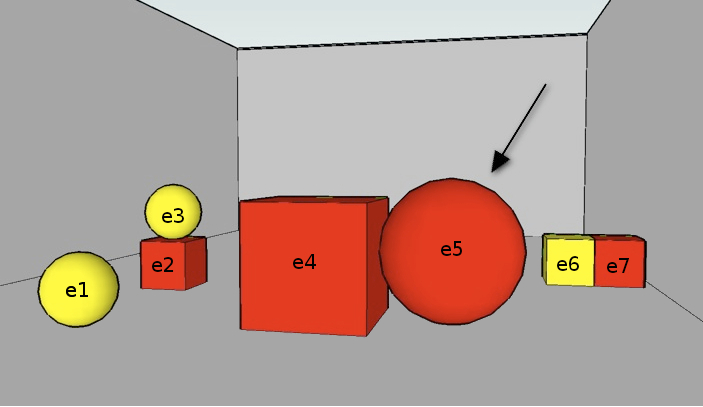
\includegraphics[width=\textwidth]{images/22.jpg}\\[0pt]
\caption{}
\label{GRE3D7-stimulus}
\vspace*{.1cm}
\end{subfigure}
\hspace*{0cm}
\begin{subfigure}{.5\textwidth}
\centering
%\vspace*{-2cm}
\begin{tabular}{l}
 {\it La esfera grande}\\
 {\it La esfera roja que est\'a al lado del cubo rojo} \\
 {\it El objeto que est\'a al lado del cubo grande}\\
 {\it La bola roja}\\
 {\it La pelota a la izquierda del cubo amarillo}\\
 {\it La bola grande}\\
 {\it La esfera que est\'a a la derecha del cubo rojo y a }\\
 {\it la izquierda del cubo amarillo}\\
 {\it La cosa que est\'a a la derecha del cubo del medio}\\
 {\it ...}
 \end{tabular}
\caption{}
\label{GRE3D7-stimulus-er}
\end{subfigure}
\caption{Expresiones referenciales para el contexto de la figura extra\'idas del GRE3D7 corpus \protect\cite{gre3d7}. En la figura los elementos se muestran etiquetados.}\label{fig2-1}

\end{figure}

De acuerdo a las propiedades o relaciones que una ER incluya, se clasifica en distintos tipos: relacional o no relacional (tambi\'en llamada proposicional), minimal, sobreespecificada, subespecificada o parcial, plural o singular. A continuaci\'on describimos cada uno de estos tipos.
% en cuyo caso es una expresi\'on que no es referencial, la incluimos en nuestras propiedades porque nos va a ser \'util la definici\'on en el Cap\'itulo \ref{sec:corpus}.\\
\begin{itemize}
\item Una ER {\bf proposicional} o no relacional, incluye s\'olo propiedades intr\'insecas del objeto target. Por ejemplo, en la Figura \ref{fig2-1}: {\it La esfera roja}. Las caracter\'isticas de ser \emph{esfera} y ser \emph{roja} son propias del objeto identificado y no de otros objetos de su contexto.

\item Una ER es {\bf relacional}, cuando contiene relaciones con otros objetos. En este caso la ER incluye descripciones de los otros objetos. Por ejemplo, en la Figura \ref{fig2-1}: {\it La esfera que est\'a a la derecha del cubo}. {\it A la derecha de} lexicaliza una relaci\'on que necesita describir otro objeto adem\'as del target, en este caso un {\it cubo}.

\item \label{sec:minimales} Se dice que una ER es {\bf minimal} cuando incluye la m\'inima cantidad de propiedades y/o relaciones con otros objetos, con las cuales el target puede ser distinguido en el contexto dado. Notar que puede haber muchas expresiones minimales. Por ejemplo, en la Figura \ref{fig2-1}: {\it La esfera roja} es una ER minimal, como as\'i tambi\'en lo es {\it La esfera grande}, y {\it La esfera a la derecha del cubo}. Para verificar que estas ERs son minimales, intentemos sacar alguna propiedad, si de {\it La esfera roja} sacamos esfera, ya no podemos identificar al target, si sacamos roja, tampoco. Lo mismo pasa para {\it La esfera grande}. Veamos que pasa con {\it La esfera a la derecha del cubo}, si sacamos {\it esfera} tenemos otro objeto, $e_7$, adem\'as del target que tambi\'en tiene a la izquierda un cubo. Si sacamos {\it a la derecha de} no es posible construir una frase nominal aceptable. 

\item Cuando la ER contiene m\'as informaci\'on de la m\'inima necesaria para distinguirlo de los dem\'as objetos en el contexto dado, se dice que la ER es {\bf sobreespecificada}. Por ejemplo: {\it La esfera roja grande} en la Figura \ref{fig2-1} es sobreespecificada porque se le puede sacar {\it grande} y sigue siendo una ER correcta, o se le puede sacar {\it roja} y tambi\'en lo sigue siendo. \label{er-sobreespecificadas}

\item Una expresi\'on\footnote{Estrictamente hablando, una expresi\'on subespecificada no es una ER dado que no identifica un\'ivocamente al target. Sin embargo, en esta tesis hablaremos en ocasiones de ERs subespecificadas para referirnos a \'estas expresiones que no alcanzan a ser referenciales.} es {\bf subespecificada} cuando no puede distinguir al target de los otros objetos en el contexto. Estos otros objetos son llamados \textbf{distractores}. Por ejemplo: {\it La esfera} en la Figura \ref{fig2-1} no alcanza a identificar al objeto $e_5$ apuntado por la flecha, ya que hay otras 2 esferas que son distractores, $e_1$ y $e_3$. Una expresi\'on subespecificada identifica a un conjunto de objetos y ese conjunto incluye otros objetos adem\'as del target.

\item Una ER es {\bf plural} cuando el target es un conjunto no singleton. Por ejemplo {\it Las esferas} es una ER para las 3 esferas de la Figura \ref{fig2-1}. {\it Las esferas} es una ER \textbf{colectiva} que con una s\'ola propiedad describe 3 objetos. Otra ER para el mismo target podr\'ia ser {\it La esfera que est\'a sola, y la que esta arriba del cubo y la que est\'a al lado del cubo rojo}, la cual es una expresi\'on \textbf{distributiva}.

\item Una ER es {\bf singular} cuando el target es singleton, es decir es un s\'olo objeto. Las ERs de la Figura \ref{fig2-1} son todos ejemplos de ERs singulares ya que el target (el objeto apuntado por la flecha) es uno solo. 

\item Una expresi\'on es {\bf parcial} cuando es una ER plural que representa a un subconjunto estricto del target. Por ejemplo, en la Figura \ref{fig2-1}, si quisieramos identificar las 3 esferas y damos la expresi\'on {\it Las esferas peque\~nas}, s\'olo identificamos a 2 de las 3 esferas requeridas.
\end{itemize}

\subsection{?`\emph{C\'omo} generamos expresiones referenciales?}
\label{sec:psicolinguistica}

?`C\'omo usamos el lenguaje para trasmitir y entender expresiones referenciales? En la teor\'ia propuesta por \cite{clark1992arenas} se asume que el hablante usa un principio de dise\~no \'optimo, es decir, los hablantes dise\~nan sus oraciones de tal manera que sus interlocutores tengan suficiente informaci\'on para entenderles, pero no m\'as de la necesaria. Para hacer esto modelan la informaci\'on que es parte del conocimiento mutuo, creencias mutuas y suposiciones mutuas. 

En la investigaci\'on \cite{keysar:Curr98} se discute que bajo ciertas condiciones los interloculores dejan de usar el principio de dise\~no \'optimo. %Cuando las 

Keysar et al. muestran muestran mediante experimentos cuidadosamente dise\~nados que, al producir expresiones referenciales, las personas no consideran el punto de vista del receptor desde el principio, sino en una etapa de revisi\'on. Es decir, los adultos producen sus ERs egoc\'entricamente, como hacen los ni\~nos, pero las corrijen antes de decirlas para que el receptor sea capaz de identificar el target un\'ivocamente.
En este trabajo se argumenta que esta primer etapa egoc\'entrica es un proceso heur\'istico que se basa en una representaci\'on de la \emph{saliencia} de las caracter\'isticas del contexto. Keysar et al. discute que una posible raz\'on para este proceso de generaci\'on heur\'istica y posterior ajuste son las limitaciones cognitivas de la mente humana. Estas limitaciones se hacen particularmente evidentes bajo restricciones de tiempo como muestran los experimentos de Keysar et al.
\emph{C\'omo} se generan las ERs, tiene un impacto en \emph{qu\'e} ERs se generan. Keysar et al. analizan que el modelo propuesto por ellos de generaci\'on-y-ajuste podr\'ia explicar en parte el tipo de sobreespecificaci\'on que se observa en las ERs generadas por personas. Durante el proceso heur\'istico inicial, la persona incluye m\'as propiedades y/o relaciones que las necesarias para identificar al target, guiada por una representaci\'on saliencia en el contexto dado.

Como dijimos, normalmente las personas cuando hablan, dan m\'as informaci\'on de la m\'inima necesaria para identificar al target, es decir sobreespecifican. Como este es un fen\'omeno tan frecuente, hay mucho trabajo relacionado. En esta secci\'on describimos el trabajo que fue relevante para el dise\~no de nuestros algoritmos que se proponen en el Cap\'itulo \ref{sec:algoritmo}. En la Secci\'on \ref{sec:link-algoritmo} explicamos de qu\'e manera este trabajo influenci\'o nuestro dise\~no.

\cite{arts} estudiaron c\'omo la sobreespecificaci\'on afecta a las personas cuando interpretan ERs. Hicieron experimentos sobreespecificando ERs ya sea con informaci\'on de las caracter\'isticas intr\'insecas de los objetos (tama\~no, color, forma) o de su ubicaci\'on (en el eje vertical u horizontal). Los resultados del experimento
proporcionaron informaci\'on sobre el efecto de la sobreespecificaci\'on en el tiempo de la identificaci\'on del target.
Concluyen que las ER sobreespecificadas conducen a una identificaci\'on m\'as r\'apida del target en contextos complejos, cuando permitieron que el lector 
tenga una imagen mental completa de la entidad. Por otro lado que delimitan la b\'usqueda a una parte m\'as espec\'ifica
del contexto. La informaci\'on adicional sobre la ubicaci\'on vertical (arriba, abajo) ha demostrado ayudar m\'as a la velocidad de reconocimiento que la informaci\'on adicional sobre el eje horizontal (izquierda, derecha).

En \cite{do-speakers} tambi\'en se estudia la sobreespecificaci\'on. En un experimento mostraron que al menos la tercera parte de los hablantes sobreespecific\'o sus ERs. Un segundo experimento mostr\'o que los oyentes no juzgan las descripciones sobreespecificadas como peores que las expresiones concisas. Y un tercer experimento, revel\'o que en contextos simples, las descripciones sobreespecificadas desencadenan movimientos oculares que pueden interpretarse como una indicaci\'on de confusi\'on. 

%Nuestras observaciones verifican \'este hecho, y veremos m\'as adelante en este cap\'itulo que en un ejemplo de la Figura \ref{GRE3D7-stimulus} m\'as del 50\% de las ER dadas por personas fueron sobreespecificadas.

\cite{Lu_sasha2015} estudiaron el rol que la cantidad de informaci\'on juega en la coordinaci\'on l\'exica en un entorno virtual interactivo. Experimentaron con 2 conjuntos de personas, a un conjunto se les dieron ERs sobreespecificadas, y al otro minimales. Concluyeron que las ERs sobreespecificadas ayudaron m\'as que las minimales a aprender palabras nuevas en idioma ruso.


Paraboni et al. en su paper \cite{acl-Paraboni15} estudian la sobreespecificaci\'on de las ERs, en particular de las ERs relacionales.
La hip\'otesis que eval\'uan es la siguiente:
\begin{it}
\begin{displayquote}h1: Dado el objetivo de sobre-especificar una descripci\'on relacional usando una propiedad p extra para el landmark, p deber\'ia corresponder a la propiedad m\'as discriminatoria que est\'a disponible en el contexto. \cite{} 
\end{displayquote}
\end{it}

Un \textbf{landmark} de un target en un contexto dado, es un objeto del contexto que est\'a relacionado con el target a trav\'es de una relaci\'on particularmente saliente. Por ejemplo en la Figura \ref{fig-2-2} el cubo rojo grande que est\'a bajo el target, es el landmark.
Una propiedad o relaci\'on es m\'as \textbf{discriminatoria} que otra cuando, al ser agregada a una ER, elimina m\'as distractores. Por ejemplo, en la Figura \ref{fig-2-2}, el tama\~no del landmark es m\'as discriminatoria que su color: agregar \emph{grande} a la expresi\'on \emph{cubo} elimina 3 distractores, mientras que agregar \emph{rojo} s\'olo elimina 2.

De acuerdo a los resultados de trabajo previo (ver \cite{Pechmann1989}) se asume que se prefiere incluir el color en una ER antes de incluir el tama\~no de un objeto. 
tama\~no de un objeto. 
Adem\'as, siguiendo el principio de dise\~no \'optimo de \cite{clark1992arenas} se supone que propiedades unarias como color o tama\~no se preferir\'an frente a relaciones que resultan en descripciones m\'as complejas. \cite{acl-Paraboni15} argumenta en contra de este trabajo previo mostrando que dependiendo s\'olamente de su poder discriminativo, se puede preferir tama\~no antes que color y se pueden preferir expresiones relacionales largas en vez de expresiones proposicionales m\'as cortas.
Ilustramos la preferencia por propiedades m\'as discriminatorias evaluando la hip\'otesis h1 usando la Figura \ref{fig-2-2}. De acuerdo a \cite{Pechmann1989} se supone que si se decide sobreespecificar el landmark en la ER \emph{la esfera sobre el cubo}, se agregar\'ia el color: \emph{la esfera sobre el cubo rojo}. Si h1 es cierto, sin embargo, se preferir\'a generar \emph{la esfera sobre el cubo grande}, porque \emph{grande} es m\'as discriminatoria que \emph{rojo} en el ejemplo. Los experimentos presentados en \cite{acl-Paraboni15} muestran que la hip\'otesis es cierta en la mayor parte de los datos analizados. Este es un resultado interesante para nuestro trabajo dado que refina el trabajo de \cite{keysar:Curr98} previamente descripto identificando el poder discriminativo de una propiedad como parte de su definici\'on de saliencia.
Esto se correlaciona con nuestros resultados y el rol del poder discriminatorio en la tarea de aprendizaje autom\'atico que describimos en el Cap\'itulo \ref{sec:algoritmo}.

La discriminaci\'on de una propiedad juega un rol central en la tarea de desambiguaci\'on. En el art\'iculo buscan probar que la discriminaci\'on tambi\'en es importante cuando no hay nada para desambiguar, como es el caso de la sobreespecificaci\'on.


%Supongamos que queremos obtener una expresión referecial para el objeto se\~nalado por la flecha en la Figura\ref{GRE3D7-stimulus7} del GRE3D7 


\begin{figure}[ht]
\centering
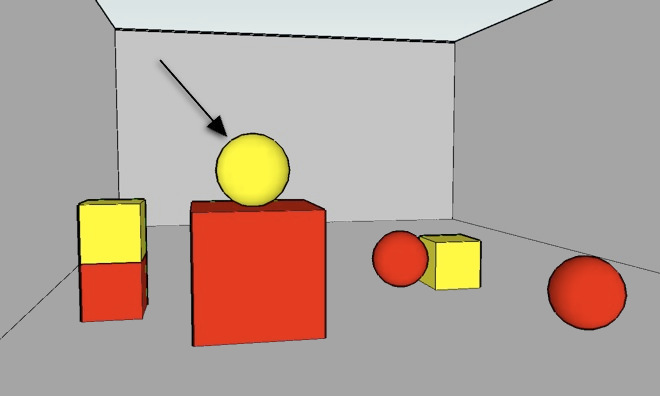
\includegraphics[width=0.6\textwidth]{images/7.jpg}
\caption{Ejemplo de contexto del corpus GRE3D7 en el que el landmark (el cubo grande), tiene una propiedad altamente discriminatoria: su tama\~no. El landmark es el \'unico objeto grande de la escena.}
\label{fig-2-2}
\end{figure}



%En nuestro trabajo para calcular las prob de uso de las palabras en el GRE3D7 , una de las propiedades fue la discriminacion, nosotros no encontramos tal correlación,  quizás por el mismo motivo q el dice (naturaleza del corpus)
%
%Me pregunto porque lo acotó a solo 1 propiedad y solo a la descripción del landmark
%Me gustaría probar q las prob de uso en el Start2, tienen fuerte correlación con la discriminacion.
%Me hubiera gustado q otro baseline en su trabajo fuera nuestro algoritmo...(me parece q tenia miedo)
%Nosotros tenemos una probabilidad de uso que nos sirve para agregar sobreespecificacion a la descripción del target y de los landmarks , no tenemos restricción de cantidad, podemos agregar varias.
%Los n\'umeros no son directamente comparables, ya q el filtro solo las relacionales y uso el total del corpus y nosotros usamos la mitad del corpus (solo verde, azul)



\subsection{Corpora de expresiones referenciales}
\label{sec:corpus2}
\label{sec:corpusTUNA}

%was the first prominent REG corpus to be made publicly available for research purposes. The corpus was developed in a series of general-purpose controlled experiments, containing 2280 descriptions produced by 60 speakers in two domains (1200 descriptions of furniture items and 1080 descriptions of people's photographs). TUNA does not contain relational descriptions, and it is possibly the only resource of this kind to include situations of reference to sets. The TUNA corpus has been extensively used in a series of shared tasks

{\bf TUNA} \cite{tuna-corpus} fue el primer corpus prominente de ERs disponible p\'ublicamente con fines de investigaci\'on. El corpus fue desarrollado en una serie de experimentos controlados de prop\'osito general, contiene 2.280 descripciones producidas por 60 personas en dos dominios (1.200 expresiones referenciales de im\'agenes de muebles y 1080 expresiones referenciales de fotograf\'ias de personas situadas en una grilla). Se muestran ejemplos de im\'agenes en la Figura \ref{imagenes-tuna}. El corpus TUNA no contiene descripciones relacionales. Este corpus se ha utilizado ampliamente en una serie de desaf\'ios \cite{reg2009}. En el Cap\'itulo \ref{sec:corpus} de esta tesis se usa para evaluar nuestros algoritmos y as\'i comparamos con el desempe\~no de otros algoritmos del \'area que participaron en estos desaf\'ios. El corpus contiene s\'olo una ER por escena, por lo cual es \'util para comparar rankings de ERs, y la evaluaci\'on de nuestro algoritmo con respecto a este corpus es limitada.


%\begin{figure}[H]
%\begin{subfigure}{.5\textwidth}
  %\centering
%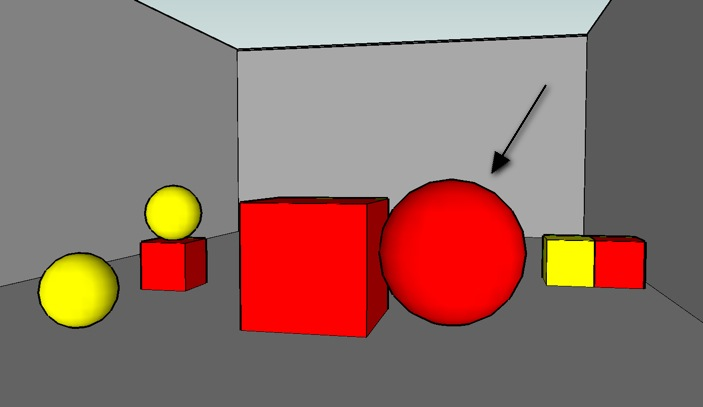
\includegraphics[width=\textwidth]{images/22sinletras.jpg}
  %\caption{}\label{GRE3D7-stimulus1}
%\end{subfigure}%
%\begin{subfigure}{.5\textwidth}




\begin{figure}[!ht]
\begin{subfigure}{.5\textwidth}
%\begin{minipage}[H]{0.5\linewidth}
\centering
\vspace*{.1cm}
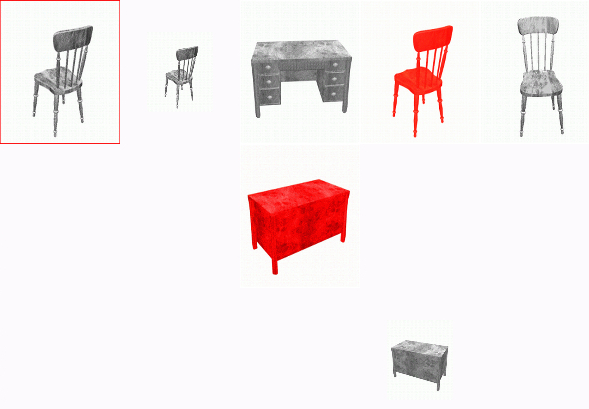
\includegraphics[width=\textwidth]{images/largeGreyChair.jpg}\\[0pt]
\caption{}
\label{fig-TUNA-furniture}
%\vspace*{.1cm}
\end{subfigure}
\hspace*{0cm}
\begin{subfigure}{.5\textwidth}
%\begin{minipage}[H]{0.5\linewidth}
\centering
\vspace*{-.8cm}
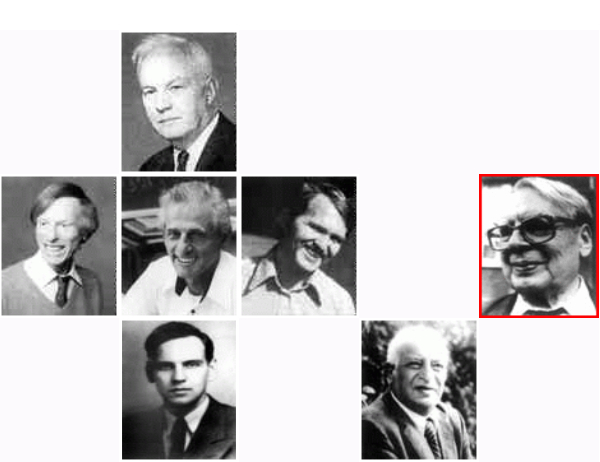
\includegraphics[width=\textwidth]{images/tuna-people.jpg}\\[0pt]
\caption{}
\label{fig-TUNA-people}
\end{subfigure}
\caption{Im\'agenes del TUNA corpus}\label{imagenes-tuna}
\end{figure}


\label{sec:corpusGRE}
%were developed in a series of web-based experiments primarily focussed on the study of relational descriptions. GRE3D3 contains 630 descriptions produced by 63 speakers, and GRE3D7 contains 4480 descriptions produced by 287 speakers, making it the largest of its kind to date. The GRE3D domain consists of simple visual scenes containing only two kinds of objects (boxes and spheres) with limited variation in colour and size. In each scene, there is only one possible spatial relation between target and the nearest landmark. Both corpora contain atomic and relational descriptions.
{\bf GRE3D3} y su extensi\'on {\bf GRE3D7} \cite{gre3d3,gre3d7} se desarrollaron en una serie de experimentos basados en la web, y se centraron principalmente en el estudio de las descripciones relacionales. GRE3D3 contiene 630 descripciones producidas por 63 personas y GRE3D7 contiene 4.480 descripciones producidas por 287 personas, y es el corpus m\'as grande del \'area hasta la fecha. El dominio de estos corpora constan de escenas visuales simples que contienen s\'olo dos tipos de objetos (cubos y esferas) con variaci\'on limitada en color y tama\~no. En cada escena, hay una relaci\'on espacial entre el target y el landmark m\'as cercano. Ambos corpus contienen descripciones proposicionales y relacionales. Ejemplo de im\'agenes del GRE3D3 y GRE3D7 se muestran en la Figura \ref{imagenes-GRE3D3-GRE3D7}. Las escenas del GRE3D3 contienen s\'olo 3 objetos mientras que las escenas del GRE3D7 contienen 7 objetos. El GRE3D7 contiene m\'as de 100 expresiones referenciales por escena. Permitiendo una evaluaci\'on detallada de los rankings que generados por nuestros algoritmos como se describe en el Cap\'itulo \ref{sec:corpus}.
%\begin{minipage}[b]{0.45\linewidth}

\begin{figure}[!ht]
\begin{subfigure}{.5\textwidth}
\centering
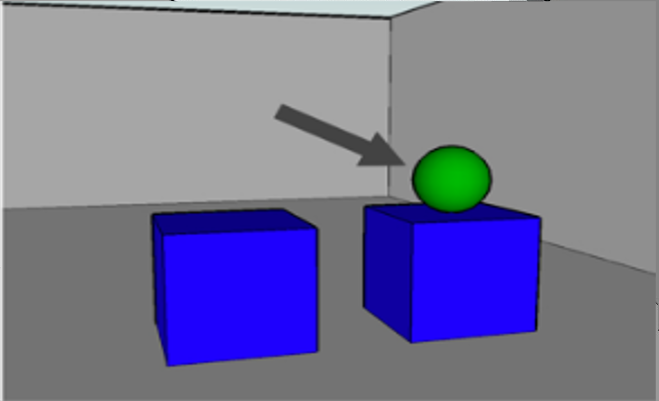
\includegraphics[width=\textwidth]{images/GRE3D3.png}\\[0pt]
\caption{}
\label{fig-GRE3D3}
%\vspace*{-0.7cm}
\end{subfigure}
\hspace*{0cm}
\begin{subfigure}{.5\textwidth}

\centering
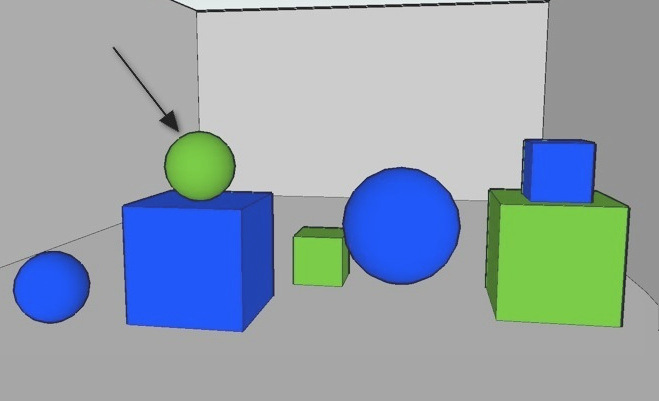
\includegraphics[width=\textwidth]{images/3.jpg}\\[0pt]
\caption{}
\label{fig-GRE3D7}
\end{subfigure}
\caption{Im\'agenes del GRE3D3 corpus (a) y del GRE3D7 corpus (b)}\label{imagenes-GRE3D3-GRE3D7}
\end{figure}

\vspace*{1cm}

\label{sec:corpusSTARS}
%and its extension Stars2 were collected for the study of referential overspecification (particularly in the case of relational descriptions). Stars was developed in a pilot web-based experiment, containing 704 descriptions produced by 64 speakers.  The more comprehensive Stars2 data set was produced in dialogue situations involving subject pairs, and it contains 884 descriptions produced by 56 speakers. Both domains make use of simple visual scenes containing up to four object types (e.g., stars, boxes, cones and spheres) with limited variation in colour and size. Differently from other REG corpora, however, Stars/2 includes a considerable number of complex situations of reference involving up to three objects, as in `the box near the sphere, next to the cone'.http://ppgsi.each.usp.br/arquivos/RelTec/PPgSI-002_2014.pdf y http://ppgsi.each.usp.br/arquivos/RelTec/PPgSI-001_2015.pdf
{\bf Stars} \cite{Paraboni2016} y su extensi\'on {\bf Stars2} se recolectaron para el estudio de la sobre-especificaci\'on (particularmente en el caso de las descripciones relacionales). Stars se desarroll\'o en un experimento piloto basado en la web, contiene 704 descripciones producidas por 64 personas. El conjunto de datos Stars2 se obtuvo de situaciones de di\'alogo que implicaban a dos personas, contiene 884 descripciones producidas por 56 participantes. Ambos dominios hacen uso de escenas visuales simples que contienen tres tipos de objetos (por ejemplo para Stars, estrellas, cuadrados y c\'irculos y para Stars2 cubos, conos y esferas) con variaci\'on limitada en color y tama\~no. A diferencia de otros corpus para GER, Stars/2 incluyen un n\'umero considerable de situaciones complejas de referencia en que participan hasta tres objetos, como en {\it el cubo cerca de la esfera, al lado del cono}. Ejemplos de im\'agenes se muestran en la Figura \ref{imagenes-stars-stars2}. Este corpus fue recientemente liberado y planeamos usarlo en trabajo futuro (ver Cap\'itulo \ref{sec:conclusiones}).

\begin{figure}[!ht]
\begin{subfigure}{.5\textwidth}

\centering
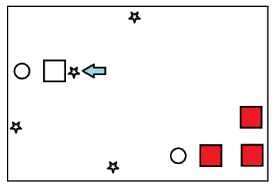
\includegraphics[width=\textwidth]{images/STARS.png}\\[0pt]
\caption{}
\label{fig-STARS}
%\vspace*{1cm}
\end{subfigure}
\hspace*{0cm}
\begin{subfigure}{.5\textwidth}

\centering
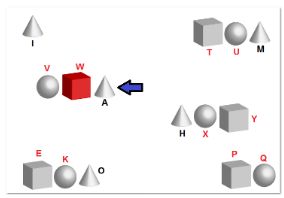
\includegraphics[width=\textwidth]{images/STARS2.png}\\[0pt]
\caption{}
\label{fig-STARS2}
\end{subfigure}
\caption{Im\'agenes del corpus Stars (a) y del corpus Stars2 (b)}\label{imagenes-stars-stars2.}
\end{figure}


\label{sec:corpusZOOM}
%were developed in a series of web-based experiments primarily focussed on the study of relational descriptions. GRE3D3 contains 630 descriptions produced by 63 speakers, and GRE3D7 contains 4480 descriptions produced by 287 speakers, making it the largest of its kind to date. The GRE3D domain consists of simple visual scenes containing only two kinds of objects (boxes and spheres) with limited variation in colour and size. In each scene, there is only one possible spatial relation between target and the nearest landmark. Both corpora contain atomic and relational descriptions.
{\bf ZOOM} \cite{DBLP:conf/acl/AltamiranoFPB15} se desarroll\'o durante nuestra colaboraci\'on con la Universidad de S\~ao Paulo. Contiene ERs para 20 mapas de las ciudades de Lisboa y Madrid, fue realizado en la web, y contiene ERs de targets singulares y plurales, con y sin zoom, en 2 idiomas: espa\~nol y portugu\'es. El corpus portugues contiene 100 ER por mapa, es decir 2000 ER en total, y el espa\~nol 80 por mapa, sumando un total de 1600 ER. El corpus fue recolectado a fin de poder realizar experimentos con situaciones m\'as cercanas a aplicaciones que los corpus existentes hasta el momento. Ejemplos de mapas se muestran en la Figura \ref{imagenes-zoom-corpus}.


%\begin{figure}[!ht]
%\begin{minipage}[b]{0.46\linewidth}
%\centering
%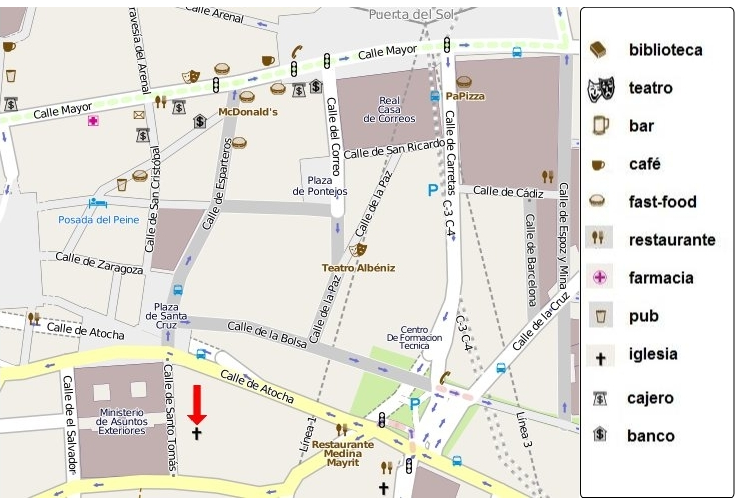
\includegraphics[width=\textwidth]{images/corpus/mapa6.png}\\[0pt]
%\caption{Target singular con zoom X}
%\label{singularx}
%\end{minipage}
%%\vspace*{.1cm}
%\begin{minipage}[b]{0.54\linewidth}
%\centering
%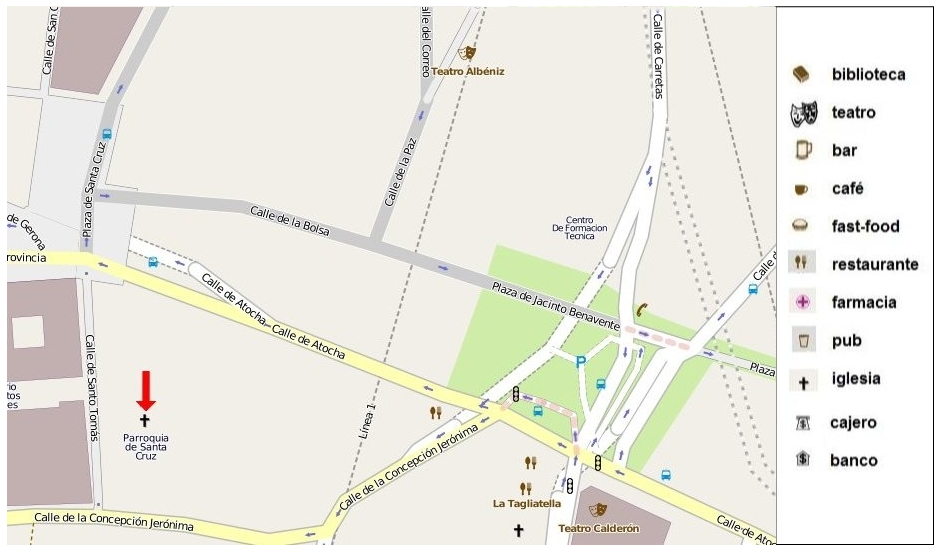
\includegraphics[width=\textwidth]{images/corpus/mapa16.png}\\[0pt]
%\caption{Target singular con zoom 2X}
%\label{singular2x}
%\end{minipage}
%\end{figure}

\begin{figure}[H]
\begin{subfigure}{.47\textwidth}
\centering
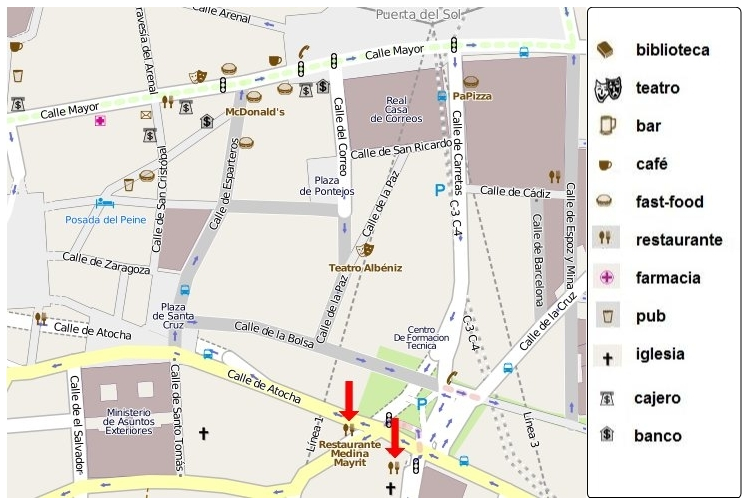
\includegraphics[width=\textwidth]{images/corpus/mapa10.png}\\[0pt]
\caption{}
\label{pluralx}
\end{subfigure}
%\vspace*{.1cm}
\begin{subfigure}{.53\textwidth}
\centering
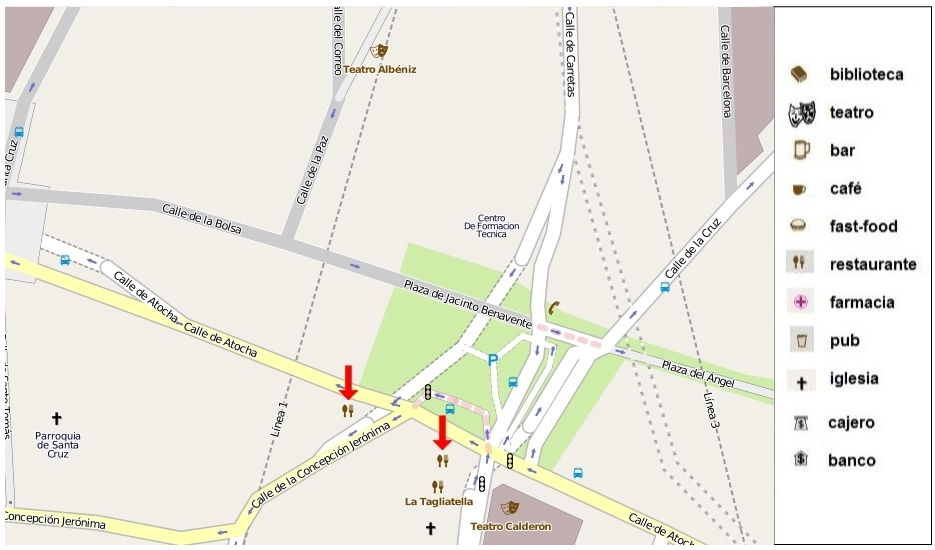
\includegraphics[width=\textwidth]{images/corpus/mapa20.png}\\[0pt]
\caption{}
\label{plural2x}
\end{subfigure}
\caption{Im\'agenes del ZOOM corpus, target plural sin zoom (a) y con zoom (b)}\label{imagenes-zoom-corpus}
\end{figure}

En la Tabla \ref{tab-comparison-prop} se comparan los diferentes corpus presentados anteriormente\footnote{En el caso del TUNA y el ZOOM se us\'o para la comparaci\'on s\'olo la parte singular.}. El n\'umero de propiedades diferentes que tiene en cuenta cada corpus se muestra en columna Propiedades. El n\'umero de posibles landmarks que la descripci\'on puede incluir se muestra en la columna Landmarks, el largo promedio de la ER, en el sentido de la cantidad de atributos y relaciones, se ve en la columna Largo promedio. Y la proporci\'on de propiedades usadas, se muestra en la columna Uso. Esta es la proporci\'on de propiedades que aparecen en la descripci\'on sobre el n\'umero total de posibles propiedades y landmarks. Mayores largos de descripci\'on y menor promedio de uso se ven en situaciones complejas de referencia. Como se puede observar, el corpus ZOOM es m\'as complejo en este sentido y es el que usamos para nuestros casos de estudio en el Cap\'itulo \ref{sec:evaluacion}.
  %the average description size (in number of annotated properties), and the proportion of property usage, which is taken to be  the proportion of properties that appear in the description over the total number of possible attributes and landmarks. From a REG perspective, larger description sizes and lower usage rates are likely to represent more complex situations of reference.

\begin{table}[ht]
\begin{center}
\footnotesize{
\caption{Compaci\'on de corpora GER existente}
\label{tab-comparison-prop}
\begin{tabular} {  l c c c c}
\hline
Corpus											&Propiedades			  & Landmarks			& Largo promedio	& Uso \\
\hline
TUNA-Muebles							  & 4								& 0							&	3.1				& 0.8   \\
TUNA-Personas								& 10							& 0							& 3.1				& 0.3   \\
GRE3D3											&	9								& 1							& 3.4				& 0.3   \\
GRE3D7											&	6								& 1							& 3.0				& 0.4   \\
Stars												&	8								& 2							& 4.4				& 0.4   \\
Stars2											& 9								& 2							& 3.3				& 0.3   \\
Zoom-Portugu\'es						& 19							& 4							& 6.7				& 0.3   \\
Zoom-Espa\~nol							& 19							& 4							& 7.2				& 0.3   \\
\hline
\end{tabular}
}
\end{center}
\end{table}

\section{Generaci\'on \emph{autom\'atica} de expresiones referenciales}
\label{sec:tipos_algoritmos}

Un algoritmo para la generaci\'on autom\'atica de expresiones referenciales es un programa que dado un contexto y un target genera una ER para el target.

Los algoritmos pueden ser de distintos tipos, seg\'un los tipos de ERs que sean capaces de generar. Por ejemplo, un algoritmo puede ser: determin\'{i}stico o no-determin\'{i}stico, relacional o proposicional, incluir negaciones o no, generar plurales, singulares o ambos,
 %usar disyunciones y conjunciones, o s\'olo conjunciones, 
generar ERs sobreespecificadas o minimales. A continuaci\'on se describen cada uno de esos tipos.

Un algoritmo es {\bf determin\'{i}stico} si dado un input (un contexto y un target), d\'a siempre la misma ER de salida. En cambio, un algoritmo es {\bf no-determin\'{i}stico} si es posible que d\'e distintas salidas para el mismo input, en distintas ejecuciones. En general las personas generan expresiones referenciales de forma no determin\'istica, en este sentido los algoritmos no-determin\'isticos simulan el comportamiento de las personas. 

Por ejemplo, un algoritmo no determin\'istico podr\'ia generar para la Figura \ref{fig2-1}, una vez {\it La esfera roja} y otra vez {\it La esfera grande}. En la Tabla \ref{er-gre3d7-stimulus} se muestran las distintas ERs dadas por las personas para la Figura \ref{fig2-1} del corpus GRE3D7 \cite{gre3d7}. La tabla tambi\'en muestra cu\'antas personas generaron esa ER para el target de la figura. Por ejemplo {\it large red ball} ocurri\'o 71 veces en el corpus, es decir m\'as de la mitad de las personas decidieron incluir el tipo, el tama\~no y el color en su ER, generando as\'i una ER sobreespecificada.

%Si el algoritmo es determin\'istico dar\'ia s\'olo una ER. ?`Esa ER que dar\'ia el algoritmo coincidir\'a con alguna de las que dieron las personas?. 
%Si el algoritmo es no-determin\'istico, ?`podremos conseguir todos los diferentes tipos de ER que dieron las personas?. %Intentaremos responder estas preguntas m\'as adelante en la tesis.\\
Si el largo de la ER es finito, dado un contexto finito, existen finitas ER a generar, as\'i un algoritmo no-determin\'istico nos permitir\'ia explorar el espacio de ERs posibles para un input dado. Tambi\'en nos permite generar un ranking de ERs como se discute en el Cap\'itulo \ref{sec:intro}.

\begin{table}[h!]
\begin{center}
\begin{tabular}{|c|l|c|}
\hline
%total scenes in evaluation set &                           80   &             68
 Orden&ER& Cantidad \\
\hline
1&large red ball & 71 \\
2&red ball & 56 \\ 
3&large red ball next-to large red cube & 5 \\ 
4&large ball & 2 \\ 
5&large red ball next-to red cube & 2 \\ 
6&large red ball right-of large red cube & 1 \\ 
7&large red ball next-to large red ball & 1 \\ 
8&large red ball next-to cube & 1 \\ 
9&red ball next-to large red cube & 1 \\ \hline
Total & &140 \\ \hline
\end{tabular}
%\vspace*{.1cm}
\caption{ER dadas por las personas para la Figura \ref{GRE3D7-stimulus} del corpus GRE3D7.} 
\label{er-gre3d7-stimulus}
\vspace*{-.5cm}
\end{center}
\end{table}

Un algoritmo es {\bf proposicional}, cuando las ERs que genera contienen s\'olo atributos del target, es decir no contiene relaciones con otros objetos ni propiedades de otros objetos. Por ejemplo, s\'olo podr\'ia generar las ERs 1, 2 y 4 de la Tabla \ref{er-gre3d7-stimulus}. Es decir, genera solamente ERs proposicionales.

Un algoritmo es {\bf relacional} si adem\'as de generar ERs proposicionales genera ERs relacionales, en cuyo caso adem\'as de generar las relaciones correspondientes deber\'a generar expresiones para \'el o los objetos relacionados. Un algoritmo relacional podr\'ia generar todas las ERs de la Tabla \ref{er-gre3d7-stimulus}. No todas las descripciones de los objetos involucrados en una ER relacional, son ERs que identifican un\'ivocamente al objeto. Por ejemplo, consideremos la ER 8, {\it La gran esfera roja a la derecha del cubo}. En este caso, {\it el cubo} es una expresi\'on que se tuvo que dar como consecuencia de incluir la relaci\'on {\it a la derecha de}. La expresi\'on {\it el cubo} no es una ER del landmark si se considera aislada porque hay otros cubos en la escena. 

En algunos contextos, por ejemplo cuando el target es el \'unico que no tiene una propiedad o relaci\'on, ser\'ia \'util un algoritmo que incluya {\bf negaciones}. Por ejemplo, para la Figura \ref{fig2-1}, la ER {\it La esfera que est\'a sola} podr\'ia ser 
una forma efectiva de referirse al objeto $e_1$ dado que es la \'unica esfera que no est\'a tocado un cubo.

Algunos algoritmos pueden generar ERs para un conjunto de objetos en el contexto considerado. Por ejemplo, para la Figura \ref{fig2-1} la ER {\it Los cubos} se refiere  al conjunto de objetos \{$e_2$, $e_4$, $e_6$, $e_7$\}. Estos algoritmos generan ER {\bf plurales}. En caso de s\'olo poder generar ERs para un target singleton se dice que el algoritmo genera s\'olo {\bf singulares}.

Un algoritmo que genera ER {\bf minimales} (introducidas en la Secci\'on \ref{sec:minimales}), es un algoritmo que d\'a ERs que contienen la m\'inima cantidad de propiedades o relaciones que se necesitan para distinguir al target. Por ejemplo, en la Tabla \ref{er-gre3d7-stimulus} las ER 2 y 4 son minimales. Normalmente, si el algoritmo es minimal y determin\'istico entonces un orden preferencial de las propiedades tomado como input hace que el algoritmo pueda decidir cu\'al ER dar en caso de tener varias minimales.

Un algoritmo que haga {\bf sobreespecificaci\'on} tiene la caracter\'istica de poder dar m\'as propiedades o relaciones con otros objetos que las m\'inimas necesarias para identificar al target. Por ejemplo, para la Figura \ref{fig2-1} la ER {\it La esfera roja, grande que esta a la derecha del cubo rojo grande} es una ER sobreespecificada porque (como ya mencionamos en la Secci\'on \ref{er-sobreespecificadas}) podr\'iamos sacarle algunas propiedades o la relaci\'on y seguir\'ia siendo una ER. Sacando {\it roja} de las propiedades del target, la expresi\'on {\it La esfera grande que esta a la derecha del cubo rojo grande} sigue siendo una ER, tambi\'en podr\'iamos sacar la relaci\'on con {\it el cubo rojo grande}, quedando {\it La esfera roja, grande} y sigue siendo una ER. Viendo la Tabla \ref{er-gre3d7-stimulus} podemos notar que la ER de mayor frecuencia, es {\it large red ball} y es una ER sobreespecificada, ya que {\it red ball} o {\it large ball}, son ERs minimales para el target de la Figura \ref{fig2-1}. En la tabla hay 58 ER minimales y 82 sobreespecificadas. Es decir, el 59\% son sobreespecificadas y el 41\% minimales.

Hay una forma trivial de que un algoritmo sobreespecifique: agregar todas las propiedades y relaciones del target con otros objetos. Por ejemplo, para la Figura \ref{GRE3D7-stimulus} la ER ser\'ia {\it Large red ball left-of (large red cube right-of large red ball)}. Pero, como vemos en la Tabla \ref{er-gre3d7-stimulus}, esto no es lo que hace la gente. En esta tesis, uno de los temas que investigamos es c\'omo hacer para el que un algoritmo sobreespecifique imitando el comportamiento humano lo m\'as posible. 

Los algoritmos no generan expresiones parciales ni subespecificadas, ya que no sirven para identificar al target. La identificaci\'on del target es el objetivo de la GER.


%\section{Algoritmos importantes en el \'area}

%interesante...
%https://www.abdn.ac.uk/ncs/departments/computing-science/tunabibl-495.php


Ahora vamos a hablar de una selecci\'on de algoritmos de generaci\'on autom\'atica de expresiones referenciales del \'area que son 
particularmente relevantes para la tesis. Para un estado del arte del \'area m\'as detallado ver \cite{survey}. En la 
Tabla \ref{clasificacion_algoritmos} se muestra una clasificaci\'on seg\'un los tipos de algoritmos que vimos en la secci\'on anterior, 
considerando si es determin\'istico o no-determin\'istico, proposicional o relacional, 
si genera negaciones, plurales, si genera sobreespecificaci\'on. Notar que si no generan sobreespecificaci\'on, generan ERs minimales.

\subsection{Primeros algoritmos}

\label{sec:algoritmos_area}

\begin{table}[b]
\begin{center}
\begin{tabular}{|l|c|c|c|c|c|c|c|}
\hline
%total scenes in evaluation set &                           80   &             68
 Algoritmos& Deter- & No-Deter & Propo- & Re- & Nega- & Plu- & Sobre- \\
 & min\'istico & min\'istico & sicional & lacional & ciones & rales & especificado \\
 %Algoritmos& Det. & No-Det. & Prop. & Rel. & Neg. & Plur. & Sob. \\
\hline
Full Brevity &Si & No&Si&No&No&No& No \\
Greedy&Si & No&Si&No&No&No& Si \\
Incremental&Si & No&Si&No&No&No& No \\
GRAPH&Si & No&Si&Si&No&Si& Si \\ \hline
%Bisimulaci\'on&Si & No&Si&Si&Si&Si& No \\ \hline
%Nuestra Propuesta&No & Si&Si&Si&No&Si& Si \\

\end{tabular}
%\vspace*{.1cm}
\caption{Clasificaci\'on de algoritmos seg\'un el tipo de ER que generan.} 
\label{clasificacion_algoritmos}
\vspace*{-.5cm}
\end{center}
\end{table}


 
%survey
%http://citeseerx.ist.psu.edu/viewdoc/download?doi=10.1.1.227.8284&rep=rep1&type=pdf


\paragraph{Full brevity:} El algoritmo {\bf Full Brevity} \cite{Dale:1989:CUR:981623.981632} genera la descripci\'on m\'as corta que 
identifica al target. Es decir, genera ERs minimales. Para hacerlo, 
busca si hay una propiedad del target que no sea propiedad de ning\'un distractor. Si no hay chequea todas las posibles combinaciones 
de 2 propiedades, si no la hay, busca de a 3 y as\'i sucesivamente. Por ejemplo para la Figura \ref{fig2-1} se fijar\'ia en las propiedades 
del target {red, ball, large}, como ninguna de ellas aisladamente identifica s\'olo al target, probar\'ia con combinaciones de 2 propiedades {\it red ball} si identifica al target, devuelve {\it red ball} y finaliza.

\paragraph{Heur\'istica Greedy:} El algoritmo de {\bf Heur\'istica Greedy} iterativamente selecciona la propiedad que elimina 
m\'as distractores, y argumentan que la propiedad seleccionada tiene el m\'as alto poder discriminativo en esa etapa. Como resultado 
no siempre genera expresiones referenciales m\'inimas. Por ejemplo para la Figura \ref{GRE3D7-stimulus} se fijar\'a que {\it ball} elimina 2 distractores {$e_{1}$, $e_{3}$}, 
{\it red} elimina 3 distractores {$e_{2}$, $e_{4}$, $e_{7}$} y {\it large} elimina 1 distractores {$e_{4}$}, entonces elegir\'a {\it red}, 
pero como no alcanza para ser ER, seguir\'a con {\it ball} que es la que elimina m\'as distractores luego de {\it red}, finalizar\'a porque 
{\it red ball} identifica al target. Supongamos que hubiera otro objeto con propiedad {\it large}, entonces {\it large} eliminar\'ia tambi\'en  
 2 distractores, entonces el algoritmo devolver\'ia {\it large red ball}, y esa ER no es minimal, es sobreespecificada.
Este algoritmo es m\'as eficiente que el Full Brevity porque encontrar la descripci\'on m\'as corta es computacionalmente caro. Aunque el 
algoritmo de heur\'istica Greedy es m\'as eficiente que el Full Brevity, pronto fue superado por el algoritmo {\it Incremental} 
y sus sucesores \cite{C92-1038,Dale95computationalinterpretations}. El algoritmo Incremental fue y sigue siendo uno de los algoritmos 
m\'as importantes del \'area, lo explicamos a continuaci\'on. 

\paragraph{Incremental:}

\begin{figure}[ht]
%\centering
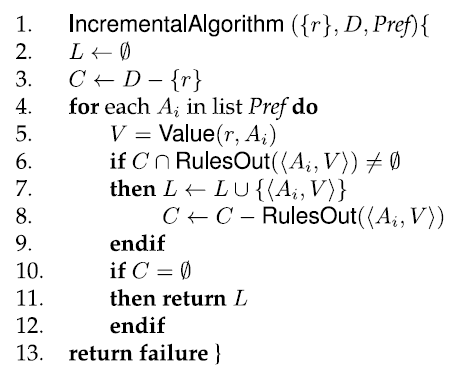
\includegraphics[width=.3\textwidth]{images/algoritmoIncremental.png}
%\caption{Algoritmo Incremental}
\label{algoritmoIncremental}
\caption{Figura 2 de \protect\cite{survey}}
\end{figure}

%\begin{figure}[ht]
%%\centering
%\includegraphics[width=0.6\textwidth]{images/algIncremental.png}
%%\caption{Algoritmo Incremental}
%\label{algoritmoIncremental}
%\caption{Figura 2 de \protect\cite{survey}}
%\end{figure}

El input del {\bf Algoritmo Incremental}, es el target \emph{r}, que queremos identificar, \emph{D} es el contexto, y \emph{Pref} una lista de propiedades ordenada seg\'un la preferencia. El algoritmo se muestra en la Figura \ref{algoritmoIncrementa}.
Vamos a ejemplificar la corrida del algoritmo con el ejemplo de la Figura \ref{fig2-1}, supongamos que el target es $e_{5}$ y la lista 
ordenada de propiedades es \'esta [tipo, color, tama\~no]. \emph{D} inicialmente es el conjunto de todos los objetos del contexto: 
\{$e_{1}$,$e_{2}$,$e_{3}$,$e_{4}$,$e_{5}$,$e_{6}$,$e_{7}$\}.
En {\it Paso 2} se asigna a \emph{L} la descripci\'on vac\'{i}a, al finalizar la ejecuci\'on, \emph{L} tendr\'a el conjunto de propiedades 
con los cuales identificaremos a $e_5$, es decir la ER. Se inicializa \emph{C} con el conjunto de distractores de \emph{r}, y $e_5$ en nuestro ejemplo \{$e_{1}$,$e_{2}$,$e_{3}$,$e_{4}$,$e_{6}$,$e_{7}$\}, en el {\it Paso 3}. 
La idea del algoritmo es ir eliminando distractores usando las propiedades $A_{i}$ del target en el orden de preferencia \emph{Pref}, por eso, en el {\it Paso 4} recorre las propiedades $A_{i}$. En {\it Paso 5} 
le asigna a \emph{V} el valor que tiene la propiedad $A_{i}$ para el target \emph{r}, en nuestro ejemplo $e_5$. $RulesOut(A_{i},V)$ es el 
conjunto de objetos que tienen 
diferente valor para la propiedad $A_{i}$ que el que tiene el target, la funci\'on se fija si el valor de esa propiedad elimina distractores. 
La primer propiedad del target $e_5$ a considerar seg\'un el orden de preferencias \emph{Pref} es el tipo, el valor del target para tipo 
es {\it esfera}. En el {\it Paso 6}, identifica los objetos en \emph{C} que tengan tipo con valor distinto de esfera, \{$e_{2}$,$e_{4}$,$e_{6}$,$e_{7}$\}, y los elimina de \emph{C}, el cual queda s\'olo con \{$e_{1}$,$e_{3}$\}. En {\it Paso 10} pregunta si \emph{C} 
es vac\'io, es decir si ya se eliminaron todos los distractores, pero no lo es, por lo tanto contin\'ua con la siguiente propiedad, 
en este caso con el color, el valor de color para el target es {\it rojo}, agrega {\it rojo} a \emph{L}, y actualiza \emph{C} con 
$\emptyset$ porque tanto $e_{1}$ como $e_{3}$ son amarillos, en {\it Paso 10} pregunta si \emph{C} es vac\'io, y si lo es, 
por lo tanto devuelve \{{\it esfera}, {\it rojo}\}. Lo cual se podr\'ia realizar como {\it La esfera roja}, y ser\'ia una ER para el target considerado.


Luego se propusieron extensiones del algoritmo Incremental, por ejemplo, una extensi\'on que permite la generaci\'on de referencia teniendo 
en cuenta la prominencia discurso del target \cite{Krahmer:2010:EMN:1880370,krahmer}; 

\paragraph{Algoritmos relacionales}

Los algoritmos que describimos hasta ahora son proposicionales. Varios investigadores han intentado ampliar el algoritmo incremental permitiendo descripciones relacionales
\cite{Horacek1997,krahmer,kelleher06:increm}, se basan a menudo
en el supuesto de que las propiedades relacionales (como ``x est\'a en y'') son menos preferidas que
los no relacionales (como ``x es blanca''), o sea que los algoritmos s\'olo las generan como \'ultima opci\'on. Si se requiere una relaci\'on para distinguir al target
x, en el cual se deba nombrar al objeto y, se aplica el algoritmo b\'asico iterativamente a y. Adem\'as, no est\'a claro que las propiedades proposicionales sean siempre preferidas antes que las relacionales. En \cite{viet:gene11} se sugieren que, incluso en escenas simples, donde los objetos pueden f\'acilmente ser distinguidos
sin relaciones, las personas tambi\'en utilizan con frecuencia las relaciones (en aproximadamente un tercio de las ERs que dan).

En caso de generar ER relacionales con esta estrategia hay que asegurarse que el algoritmo termina, es decir que no entra en ciclos infinitos 
tratando de identificar objetos. \cite{haddock} estudiaron como abordar el problema de regresi\'on infinita, en el cual el algoritmo trata de describir al landmark haciendo referencia al target, y al target haciendo referencia al landmark infinitamente, como en {\it el libro en la mesa la cual soporta un libro en la mesa... }


\subsection{Algoritmo de b\'usqueda en Grafo}
\label{graph}

%\begin{figure}[ht]
%\centering
%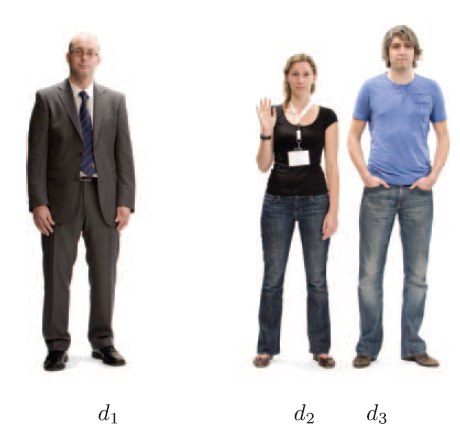
\includegraphics[width=0.4\textwidth]{images/contexto-survey.png}
%\caption{Ejemplo de contexto}
%\label{figura-survey}
%\end{figure}
%
%\begin{figure}[ht]
%\centering
%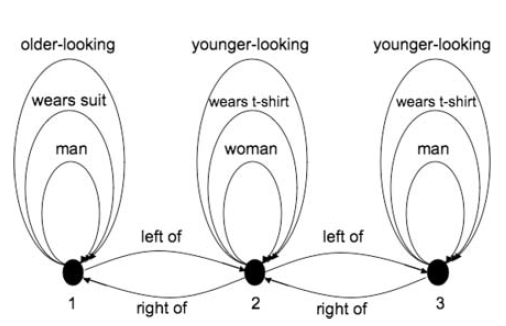
\includegraphics[width=0.4\textwidth]{images/grafo-survey.png}
%\caption{Ejemplo de grafo para el contexto de la Figura \ref{figura-survey}}
%\label{grafo-survey}
%\end{figure}


El {\bf algoritmo Graph} de \cite{graph} propone tratar la obtenci\'on de expresiones referenciales como un problema de grafos, el contexto que incluye al target y los distractores es representado como un grafo, por ejemplo para el contexto de la Figura \ref{figura-survey} el grafo correspondiente ser\'ia el de la Figura \ref{grafo-survey}. Cada objeto de la escena (personas en este caso) se modela como un v\'ertice en el grafo. Las propiedades at\'omicas como jounger-looking, older-looking, wears suit, wears t-shirt, woman, man, se representan como un bucle en el correspondiente nodo. Las relaciones binarias entre objetos, por ejemplo left-of o right-of se modelan como aristas entre los nodos correspondientes.

\begin{figure}[!ht]
\begin{subfigure}{.35\textwidth}\centering
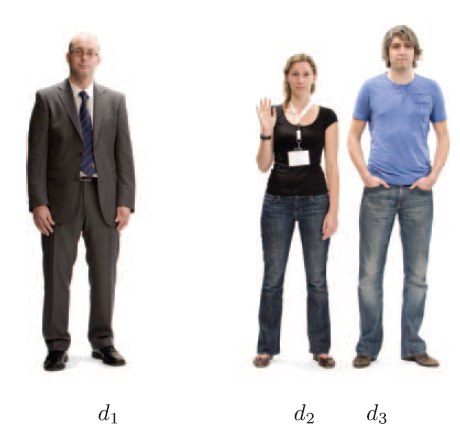
\includegraphics[width=\textwidth]{images/contexto-survey.png}\\[0pt]
%\caption{}
\label{figura-survey}
\vspace*{.1cm}
\end{subfigure}
\hspace*{0cm}
\begin{subfigure}{.55\textwidth}\centering
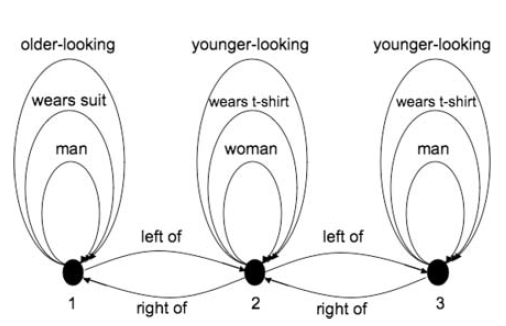
\includegraphics[width=\textwidth]{images/grafo-survey.png}\\[0pt]
%\caption{Ejemplo de grafo para el contexto de la Figura \ref{figura-survey}}
\label{grafo-survey}
\end{subfigure}
\caption{Ejemplo de contexto y grafo extra\'ido de \protect\cite{survey}}\label{fig2-8}

\end{figure}



Dado un objeto target, conseguir una ER que distinga al objeto de lo dem\'as es equivalente a encontrar un subgrafo del grafo original que unicamente caracterize al target. Intuitivamente este subgrafo se puede poner sobre el target y no sobre ningun otro objeto del dominio considerado.\\

\begin{figure}[ht]
\centering
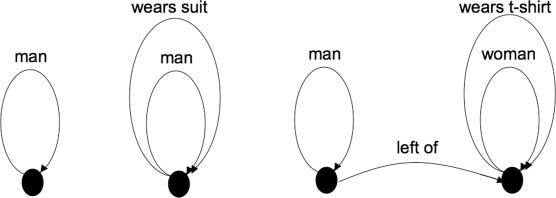
\includegraphics[width=0.6\textwidth]{images/ref-exp-graph.png}
\caption{Subgrafos de la Figura \ref{fig2-8}}
\label{ref-exp-graph}
\end{figure}

%Para generar una descripci\'on distintiva, el algoritmo busca un subgrafo del grafo original que identifica al target un\'{i}vocamente al cual le llama grafo distintivo.% (distinguishing graph).\\
Comenzando con el subgrafo que contiene un solo v\'ertice, que representa al target, seg\'un una heur\'{i}stica basada en costos (costo de incluir propiedades, relaciones) empieza a agregar propiedades o relaciones, del target o nodos que ya hallan sido agregados. Cada vez que agrega algo, chequea si hay alg\'un otro nodo en el cual el grafo pueda distinguir, si lo hay quiere decir que es un distractor, cuando no hay el grafo distingue al target. Por ejemplo en la Figura \ref{ref-exp-graph} se ve el primer grafo {\it man}, el cual puede ser puesto sobre los nodos 1 y 3 de la Figura \ref{grafo-survey}, es decir no identifica s\'olo al target, el segundo grafo {\it man, wears suit} s\'olamente puede ser puesto sobre el nodo 1, por lo tanto es un grafo que distingue al target.  

El algoritmo sigue explorando grafos y siempre se queda con el de menor costo.

La funci\'on de costo esta definida sobre las aristas y v\'ertices del grafo dominio. El costo de un subgrafo se define como la suma sobre todas las aristas y v\'ertices que contiene el grafo.
El algoritmo de b\'usqueda garantiza encontrar el subgrafo de menor costo que representa al target.

La funci\'on de costo es usada para podar las ramas del \'arbol de b\'usqueda cuando estas se hacen m\'as costosas que el grafo de menor costo encontrado hasta el momento. Esta funci\'on hace que se prefieran propiedades sobre otras que tienen mayor costo.

%Por ejemplo, 
%Los algoritmos discutidos por Dale y Reiter (1995) pueden ser vistos como
%diferentes instancias de un algoritmo de b\'usqueda (Bohnet y Dale 2005; Gatt de 2007).
%Todos ellos, b\'asicamente, buscan a trav\'es de un mismo espacio de estados, compuestos por tres componentes: conjunto de cosas verdaderas para el target, un conjunto de distractores, y un conjunto de propiedades del target que a\'un no han sido consideradas. El estado inicial se puede formalizar como la tripla ($\emptyset$, C, P) 
%(no hay descripci\'on del target constru\'ida, no se han descartado distractores, y todas las propiedades P del target todav\'ia est\'an disponibles), y el estado final como
%(L, $\emptyset$, P'), se ha encontrado una descripci\'on que distingue al target,
%el conjunto de distractores est\'a vac\'io, y pueden o no quedar propiedades del target en P'. Todos los otros estados en el espacio de b\'usqueda son intermedios,
%a trav\'es de cuales un algoritmo podr\'ia moverse en funci\'on de su estrategia de b\'usqueda. 
%Por ejemplo 
%cuando buscamos de una descripci\'on distintiva de $e_{5}$ del Contexto\ref{GRE3D7-stimulus2}, un estado intermedio podr\'ia ser
%s = ({[forma, esfera],[color,rojo]},{$e_{5}$}, {[taman\~o, grande],[a-la-der-de, $e_4$]})
%
%Los algoritmos discutidos anteriormente difieren en el m\'etodo de creaci\'on de los estados, y en el orden en que estos estados son recorridos. Full Brevity, por ejemplo, utiliza un m\'etodo de expansi\'on, que crea un nuevo estado para cada atributo
%del target no contemplado antes (y que excluye al menos un distractor). 
%
%
%Comenzando desde el estado inicial y aplicando a nuestro ejemplo de contexto, este m\'etodo ser\'ia dar\'ia lugar a tres nuevos estados, la creaci\'on de descripciones, incluyendo la informaci\'on de forma, el color, y el taman\~o, respectivamente. Estos estados son chequeados mediante un m\'etodo de amplitud-primero. 
%El IA, por el contrario, utiliza un m\'etodo diferente para ampliar el grafo, cada vez que crea
%un nuevo estado, lo hace de acuerdo con un orden de preferencia predeterminado. As\'i, en
%el estado inicial, y suponiendo que (como antes) que escribe es el atributo m\'as preferido, el
%ampliar m\'etodo ser\'ia crear un solo nuevo estado: s = {[forma, esfera]}, siempre hay 1 solo nuevo estado elegido por el orden de preferencia.



%Considere dos descripciones de un dominio de los animales ... (van Deemter, 2002), van Deemter considera integridad l\'ogica del ia en t\'erminos de los operadores booleanos de negaci\'on y disyunci\'on. \'el la extendi\'o a
%ser capaz de generar expresiones referenciales que contienen propiedades, tales como Ejemplo (2.3) negado, y las descripciones de conjuntos de objetos, tales como Ejemplo (2.4), o incluso (2,5), que contiene una disyunci\'on l\'ogica de propiedades. Sus algoritmo procede
%en etapas, tratando m\'as y disyunciones m\'as largos de propiedades, si las propiedades at\'omicas
%y disyunciones m\'as cortos no son suficientes para distinguir el conjunto target .. que funciona en referencia a conjuntos fue tomada adem\'as por Gatt y van Deemter (2005, 2006), que han presentado los algoritmos m\'as maduros a la fecha. Utilizaron un procedimiento similar al de las otras cosas en que sus algoritmos se basan en el procesamiento incremental de un orden de preferencia de las propiedades. Sus algoritmos agregan una gran cantidad de maquinaria compleja para el procedimiento b\'asico para asegurar que las propiedades
%se eligen de manera que maximiza la coherencia dentro del conjunto de objetos descritos por las expresiones referenciales. Por ejemplo, su enfoque intentar\'a utilizar propiedades del mismo tipo para todos los referentes de un conjunto. As\'i, ser\'ia producir
%descripciones tales como ejemplos
%(2.6) or (2.7) rather than Example (2.8) or.. 


%Theune y Krahmer propusieron una extensi\'on que permite la generaci\'on de referencia con la subsiguiente ia teniendo en cuenta la prominencia discurso del referente objetivo (Krahmer y Theune, 1998; Theune, 2000; Krahmer y Theune, 2002), y un segundo uno que permite la IA para producir expresiones referenciales que contener relaciones binarias a otros objetos (Theune, 2000; Krahmer y Theune, 2002). Voy a volver a su extensi\'on relacional en la Secci\'on 2.3. Enfoque Theune y de Krahmer funciona asignando una puntuaci\'on de relevancia a todos los objetos de acuerdo con la enfoque / tema distinci\'on por Hajicova (1993) y el centrado Theory (Grosz et al., 1995). Alteran el criterio de \'exito del algoritmo y s\'olo permiten que se detenga cuando aqu\'i hay izquierda distractor que es tan o m\'as relevante que el referente de destino.
%No todas las propiedades son las mismas. Las Diferencias cualitativas que existen entre diferentes propiedades se discutieron por primera vez en la literatura reg por van Deemter (2000, 2006). Se\~nal\'o que la conveniencia de propiedades orgradable vagos como peque\~nos y grandes depende del contexto en el que se utilizan, mientras que, Por ejemplo, el color de un objeto es absoluta. Considere dos descripciones de un dominio de los animales ... (van Deemter, 2002), van Deemter considera integridad l\'ogica del ia en t\'erminos de los operadores booleanos de negaci\'on y disyunci\'on. \'el la extendi\'o a ser capaz de generar expresiones que se refieren que contienen propiedades, tales como Ejemplo (2.3) negado, y las descripciones de conjuntos de objetos, tales como Ejemplo (2.4), o incluso (2,5), que contiene una disyunci\'on l\'ogica de propiedades. Sus algoritmo procede en etapas, tratando m\'as y disyunciones m\'as largos de propiedades, si las propiedades at\'omicas y disyunciones m\'as cortos no son suficientes para distinguir el conjunto de destino .. que funciona en referencia a conjuntos fue tomada adem\'as por Gatt y van Deemter (2005, 2006), que han presentado los algoritmos m\'as maduros en este espacio para la fecha. Utilizaron un procedimiento similar al de las otras cosas en que sus algoritmos se basan en el procesamiento incremental de un orden de preferencia de las propiedades. Sus algoritmos agregar una gran cantidad de maquinaria compleja para el procedimiento b\'asico para asegurar que las propiedades se eligen de manera que maximiza la coherencia dentro del conjunto de objetos descritos por las expresiones que se refieren. Por ejemplo, su enfoque intentar\'a utilizar propiedades del mismo tipo para todos los referentes de un conjunto. As\'i, ser\'ia producir Ejemplos descripciones tales como (2,6) o (2,7) en lugar de Ejemplo (2.8) o ..
En lo que sigue veremos como evaluar a los algoritmos de generaci\'on de ER.





\section{Evaluaci\'on y comparaci\'on con corpus}

\label{sec:metricas_evaluacion}

%La investigaci\'on presentada en \cite{viethen-phd} se basa en dos premisas fundamentales: que la investigaci\'on
%en la generaci\'on autom\'atica de expresiones referenciales debe esforzarse por lograr
%sistemas que den salidas tan similar a la humana como sea posible; y que, para ello, debemos
%esforzarnos para modelar el comportamiento humano como se puede observar en corpora. Nosotros adherimos a esta postura, en esta tesis se han presentado corpora existente, y vamos a evaluar nuestros resultados por un lado compar\'andolos con las ER que est\'an en los corpus, luego veremos que \'esta manera de evaluar no es del todo justa para los algoritmos, y haremos otras clases de evaluaciones para mostrarlo.
Esta secci\'on est\'a dividida en 3 partes, en la primera se muestra trabajo previo usando corpora relevante a nuestro estudio, en la segunda se explican algunas m\'etricas autom\'aticas y en la tercera se d\'a una introducci\'on a las m\'etricas manuales.

\subsection{Trabajo previo en evaluaci\'on usando corpora}\label{sec:2_3_1}
%
%La adopci\'on de estas premisas sirve para dos fines: en primer lugar, mejora la adecuaci\'on
%de la salida de algoritmos de GER para el objeto target imitando la capacidad humana
%de producir referencias adecuadas; y en segundo lugar, el estudio de corpus de datos producidos por humanos
 %y algoritmos en desarrollo que pueden replicar estos datos podr\'ian
%acercarnos a la comprensi\'on de que es lo que hacen los humanos cuando dan una ER.

%\cite{viethen-phd} dice que el cl\'asico algoritmo de GER y la mayor parte de sus descendientes no se basaron ni evaluaron contra datos producidos por humanos. Ellos se basaron en una visi\'on bastante minimalista de lo que se necesita
%para que una expresi\'on referencial sea \'optima, concentr\'andose en la eficiencia computacional 
 %y descripciones breves como sus principales preocupaciones.
%
 %Existe un peque\~no n\'umero de enfoques que 
 %se basaron en observaciones del comportamiento de referencia general humana
%que obtuvieron a partir de experimentos psicoling\"u\'isticos, pero de nuevo no fueron evaluados
%contra datos humanos.
%
%Los algoritmos que se presentaron a los desaf\'ios de evaluaci\'on \cite{gatt-balz-kow:2008:ENLG} y \cite{reg2009}
%fueron probados en el TUNA-Corpus, y algunos de ellos
%tambi\'en tuvieron en cuenta corpus del conjunto del desarrollo. Pero hay una serie de preocupaciones en torno a la pregunta de si el TUNA-Corpus, y la forma de salida de los sistemas que se compar\'o en los desaf\'ios eran ideales para una evaluaci\'on de la adecuaci\'on descriptiva de GER.
%saque esto porque no se entiende
%A partir de los desaf\'ios que se describen en m\'as detalle y para evaluarlos en una serie de datos m\'as grande
%que contiene m\'as de una expresi\'on referencial para cada elemento est\'imulo.

%No se pretend\'ia que ninguno de los algoritmos de la prueba tomara en cuenta las variaciones entre-hablantes, ni del mismo hablante. Hay implementaciones del IA que han comenzado a agregar modelo de preferencias de hablante en alg\'un grado.
%
Los temas generales que con la evaluaci\'on basada en corpus de la experiencia de \cite{viethen-phd} quedaron
al descubierto fueron (1) la interdependencia estrecha entre algoritmos y la
representaci\'on subyacente de conocimiento que utilizan, (2) el no-determinismo de la generaci\'on del lenguaje natural, 
(3) la cuesti\'on de c\'omo comparar la salida algoritmos con los gold-standar, y (4) la independencia dominio espec\'ifico deseada para los algoritmos de GER.\\
La discusi\'on de estos temas ha dado lugar a la siguiente lista de evaluaci\'on en GER basada en corpus:

i. Si el corpora est\'a destinado para ser reutilizado para la evaluaci\'on comparativa de diferentes
algoritmos, una representaci\'on subyacente del dominio, es decir de la sem\'antica, debe ser proporcionada para ser usada por todos los algoritmos.

ii. El corpus debe contener tantos casos como sea posible de tantos diferentes hablantes como sea posible para cada escenario referencial para identificar las potencialidades del contexto. 

iii. Si la probabilidad de un algoritmo de ser un modelo de la conducta humana de referencia
se eval\'ua, deben utilizarse m\'etricas basadas en cobertura y precisi\'on. Es decir, el conjunto completo de las descripciones que el algoritmo proporciona para cada
escenario de referencia en virtud de cualquier ajuste de par\'ametro debe ser comparado con el
conjunto de las descripciones contenidas en el corpus para el mismo escenario referencial.

iv. Algoritmos que son juzgados en un dominio espec\'ifico, no se debe asumir como
f\'acilmente adaptable a otros dominios. Los algoritmos deben ser evaluados en distintos dominios.

Investigaci\'on GER Pre-2000 di\'o poca o ninguna atenci\'on a la evaluaci\'on emp\'irica de los algoritmos. M\'as 
recientemente, sin embargo, los estudios de evaluaci\'on GER han comenzado a usar corpora para evaluar.

En esta secci\'on, se discuti\'o cu\'ales son los criterios que se deben cumplir
para evaluar adecuadamente los algoritmos GER.

Para medir la performance de los algoritmos podemos usar m\'etricas autom\'aticas o m\'etricas manuales, las m\'etricas autom\'aticas son aquellas que se calculan mediante un algoritmo y las manuales en las cuales les requerimos a personas que evaluen las expresiones referenciales como se describe en las siguientes secciones.


\subsection{M\'etricas autom\'aticas}
\label{sec:metricasAutomaticas}

Una de las formas m\'as usadas de evaluaci\'on son las siguientes m\'etricas que se pueden calcular autom\'aticamente con respecto a corpora.
Una m\'etrica autom\'atica de evaluaci\'on implica comparar la ER dada por el sistema para un target en un contexto dado con la ER (gold standar) dada por una persona para el mismo target y contexto.
Esta comparaci\'on de ER puede estar dada a distintos niveles, podemos comparar si son iguales, si solo difieren en el orden de las palabras, si difieren en las palabras pero no en la cantidad de palabras que contienen, etc. En lo que sigue nombramos las m\'etricas de evaluaci\'on autom\'atica m\'as usadas.

La \textbf{exactitud} ({\it accuracy}) se define como el porcentaje de coincidencias exactas entre cada ER producida por un ser humano y la producida por el sistema para la misma escena y target. Se considera que es una m\'etrica demasiado estricta.

El coheficiente \textbf{Dice} es una m\'etrica de comparaci\'on de conjuntos, el valor va entre 0 y 1, 1 indica un perfecto matcheo entre los conjuntos. Para dos ERs A y B, Dice se calcula como sigue:\\

$Dice(A,B) = \frac{2\times|A \cap B|}{|A|+|B|}$\\

\textbf{\textsc{masi}} de \cite{masi}~es un coheficiente que var\'ia en favor de la similaridad cuando un conjunto es un subconjunto de otro, como Dice varia entre 0 y 1, 1 indica matcheo perfecto. Se calcula como sigue:\\
%which biases it in favor of similarity where one set
%is a subset of the other. Like Dice, it ranges between
%0 and 1, where 1 indicates a perfect match. It is computed as follows:\\

$\textsc{masi}(A,B) = \delta \times \frac{|A \cap B|}{|A \cup B|}$ \\


donde $\delta$ es un coheficiente definido como sigue:\\


 \begin{equation}
     \delta  = \left\{
	       \begin{array}{ll}
		 0      & if A \cap B = \emptyset \\
		 1 & if A = B  \\
		 \frac{2}{3}     & if A \subset B ~or~ B \subset A\\
		 \frac{1}{3}     & otro caso
	       \end{array}
	     \right.
 \end{equation}

Intuitivamente significa que se prefieren aquellas descripciones producidas por el sistema las cuales no incluyen atributos que los humanos no incluyeron.

Notar que estas m\'etricas no cumplen con el punto (iii) de la Secci\'on \ref{sec:2_3_1} y no nos permiten compararrankings de ERs, pero igualmente las usamos en el Cap\'itulo \ref{sec:evaluacion} para poder compararnos con trabajo previo.

\subsection{M\'etricas manuales}

Las ERs tambi\'en pueden ser evaluadas por jueces humanos, y de esta manera se pueden evaluar por ejemplo adecuaci\'on, mostr\'andole a un juez humano la misma im\'agen que vi\'o la persona que gener\'o la ER y pregunt\'andole cosas como ?`Que tan clara es la descripci\'on?.
Hicimos una evaluaci\'on manual en la que pedimos a 2 jueces que elijan cual ER les es m\'as natural, se les mostro el contexto, y se les present\'o 2 ER una dada por el sistema y otra proveniente del corpus dada por un humano. Tambi\'en se le podr\'ia mostrar la misma im\'agen pero sin la flecha que se\~nala al target, darle la ER que di\'o alguna persona, y pedirle que se\~nale el objeto al cual la ER refiere. De esta manera se puede evaluar facilidad de encontrar objetivo con la expresi\'on dada.
La fluidez de una ER se puede evaluar preguntando a juez humano cosas como estas: 
?`Considera que es fluida esta descripci\'on?, ¿Es buena y clara en el idioma considerado?. 
Otra manera de evaluar manualmente es viendo si las ERs son \'utiles para dar instrucciones. Por ejemplo, \cite{BelzGattEvaluation}, mostraron a los participantes una descripci\'on generada para un ensayo. Despu\'es que los participantes le\'ian esta descripci\'on, una escena aparec\'ia y se pidi\'o a los participantes
hacer clic en el objetivo previsto. Esto les permiti\'o calcular tres m\'etricas de evaluaci\'on: %extr\'inseca
el tiempo de lectura, el tiempo de identificaci\'on, y la tasa de error, que se definen como el n\'umero de objetivos identificados incorrectamente.


\section{Notas finales y linkeo del cap\'itulo}
\label{sec:linkeo2}

Este cap\'itulo lo dividimos en 3 secciones, en la primer secci\'on dimos definiciones b\'asicas que usaremos a lo largo de toda la tesis, 
como son los tipos de ER de acuerdo a las propiedades o relaciones que incluyan, tambi\'en de acuerdo a la cantidad de informaci\'on que 
tengan, luego presentamos las premisas en las que se basa la teor\'ia de \cite{clark1992arenas,Clark-Marshall81}, vimos experimentos que muestran que dadas ciertas condiciones las personas no siguen esas premisas, 
\cite{keysar:Curr98}. Tambi\'en vimos que algo com\'un es que las personas den ERs sobreespecificadas, \cite{arts,do-speakers}, los experimentos 
indican que por lo menos la tercera parte de las expresiones son sobreespecificadas, y que los oyentes no juzgan estas ERs como peores que 
la minimales. Otras conclusiones encontradas son que la sobreespecificaci\'on permite la identificaci\'on m\'as r\'apida del target y que la 
informaci\'on adicional (arriba, abajo) es m\'as \'util que la (izquierda, derecha). \cite{Lu_sasha2015} hicieron un experimento de 
aprendizaje de palabras en una lengua extranjera, y concluyen que las personas que tuvieron a su disposici\'on ERs sobreespecificadas, 
aprendieron m\'as que aquellas a las que se les di\'o ERs minimales. Tambi\'en dimos una introducci\'on a corpora existente en el \'area 
como son el TUNA, el GRE3D3/7, Stars/2 y el ZOOM corpus que fue creado en el desarrollo de esta tesis, por lo cual lo explicaremos con m\'as detalle en el Cap\'itulo \ref{sec:corpus}. En la segunda secci\'on explicamos los diferentes tipos de algoritmos los cuales se 
diferencian por los tipos de ER que pueden generar, dimos los algoritmos m\'as importantes del \'area como son incremental, graph, relacional, vimos sus diferencias y pudimos compararlos entre ellos. Entre los algoritmos del \'area no inclu\'imos el de 
bisimulaci\'on del cual hablaremos en la Secci\'on \ref{sec:bisimulacion} por ser \'este el algoritmo base de los aportes de esta tesis. Y 
en la tercer secci\'on dimos una introducci\'on a las m\'etricas de evaluci\'on tanto autom\'aticas como manuales, algunas de las cuales usaremos para evaluar nuestro algoritmo.

